\subsection{Top quarks (Marta)}
At LHC energies the dominant production channel for top pair production is gluon-gluon fusion which is responsible for 80\%-95\% of the total pair production. The remaining $\mathrm{t}\bar{\mathrm{t}}$ pairs are from quark-antiquark annihilation. 

As discussed in \cite{d'Enterria:2015jna}, top measurements probe the nuclear gluon density in an unexplored kinematic regime around Bjorken-x values, $x \sim 2m_{\mathrm{t}}/\rootsNN \sim 5 \cdot 10^{-3}-0.05$, and virtualities $Q^{2} \sim m_{\mathrm{t}}^{2} \sim 3 \cdot 10^{4}$ GeV, a region characterized by anti-shadowing corrections. High accuracy measurements of the perturbative $\mathrm{t}\bar{\mathrm{t}}$ cross section in pp collisions, have provide a strong constraint on existing NNLO PDF sets, in particular on the large-x gluon PDF \cite{Czakon:2013tha}. A measurement of the $\mathrm{t}\bar{\mathrm{t}}$ cross section as function of pseudorapidity in pPb collisions will constrain the modificaiton of the nuclear gluon PDF in the same x-range which corresoponds to the x-range which is currently unconstrained. The top quark cross section is expected to be increased at midrapidity due to anti-shadowing while at backward rapidities ($\eta_{t}<-1.5$) large-x region is reached and the EMC effect takes over \cite{d'Enterria:2015jna}.
\begin{figure}[h!]
\begin{center}
  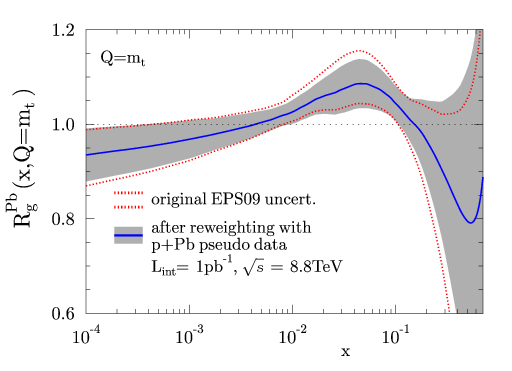
\includegraphics[width= 0.43\textwidth]{figures/top/gluons2.png}
  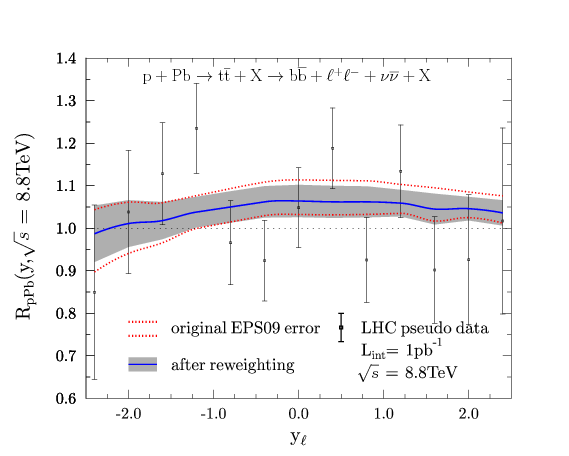
\includegraphics[width= 0.43\textwidth]{figures/top/data2.png}
  \caption{Estimated impact on the nuclear gluon of nulear modification factor measurment of $\mathrm{t}\bar{\mathrm{t}}$ decay leptons in pPb collisions at $\rootsNN=8$ TeV. Figures taken from \cite{d'Enterria:2015jna}.
  }
\label{fig:ttnPDF}
\end{center}
\end{figure}

Fig. \ref{fig:ttPPbProjections} shows the expected number of $\mathrm{t}\bar{\mathrm{t}}$ pairs (left panel) and corresponding statistical uncertainty (right panel) as function of total integrated luminosity. The total number of top pairs is calculated as follows:
\begin{equation}
N_{\mathrm{t}\bar{\mathrm{t}}} = \sigma_{\mathrm{t}\bar{\mathrm{t}}} \cdot A \cdot \mathcal{B} \cdot \mathcal{L}_{\mathrm{int}} \cdot \mathcal{A} \cdot \epsilon,
\end{equation}
with $\mathrm{t}\bar{\mathrm{t}}=244$ pb corresponding to the measurement in 8 TeV pp collisions \cite{Khachatryan:2016mqs}, A the mass number of lead (208), $\mathcal{B}$ the branching ratio corresponding to the selected final state, $\mathcal{L}_{\mathrm{int}}$ the total integrated luminosity, $\mathcal{A}$ the fraction of events within the CMS acceptance and $\epsilon$ the typical reconstruction efficiency in the CMS detector.
\begin{figure}[h!]
\begin{center}
  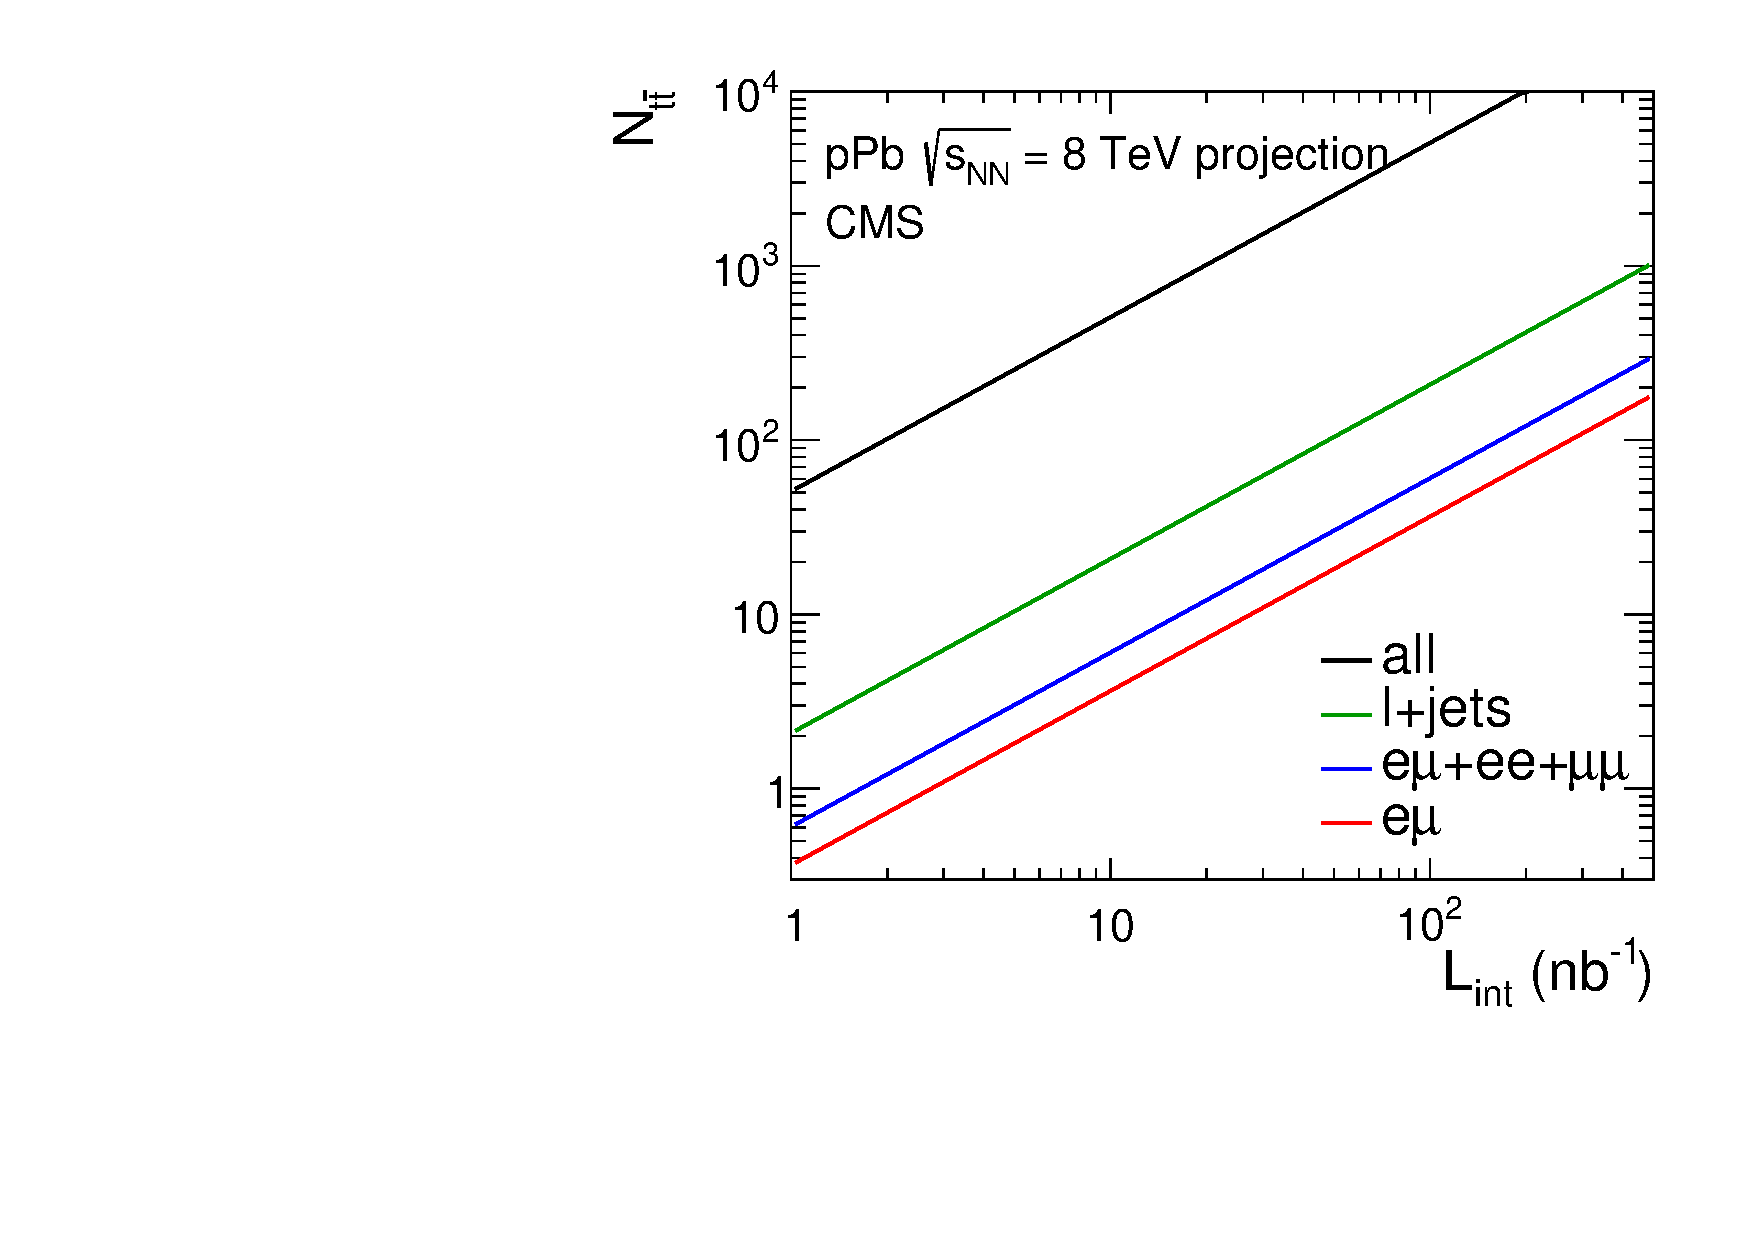
\includegraphics[width= 0.43\textwidth]{figures/top/ProjectedTTbarYield.pdf}
  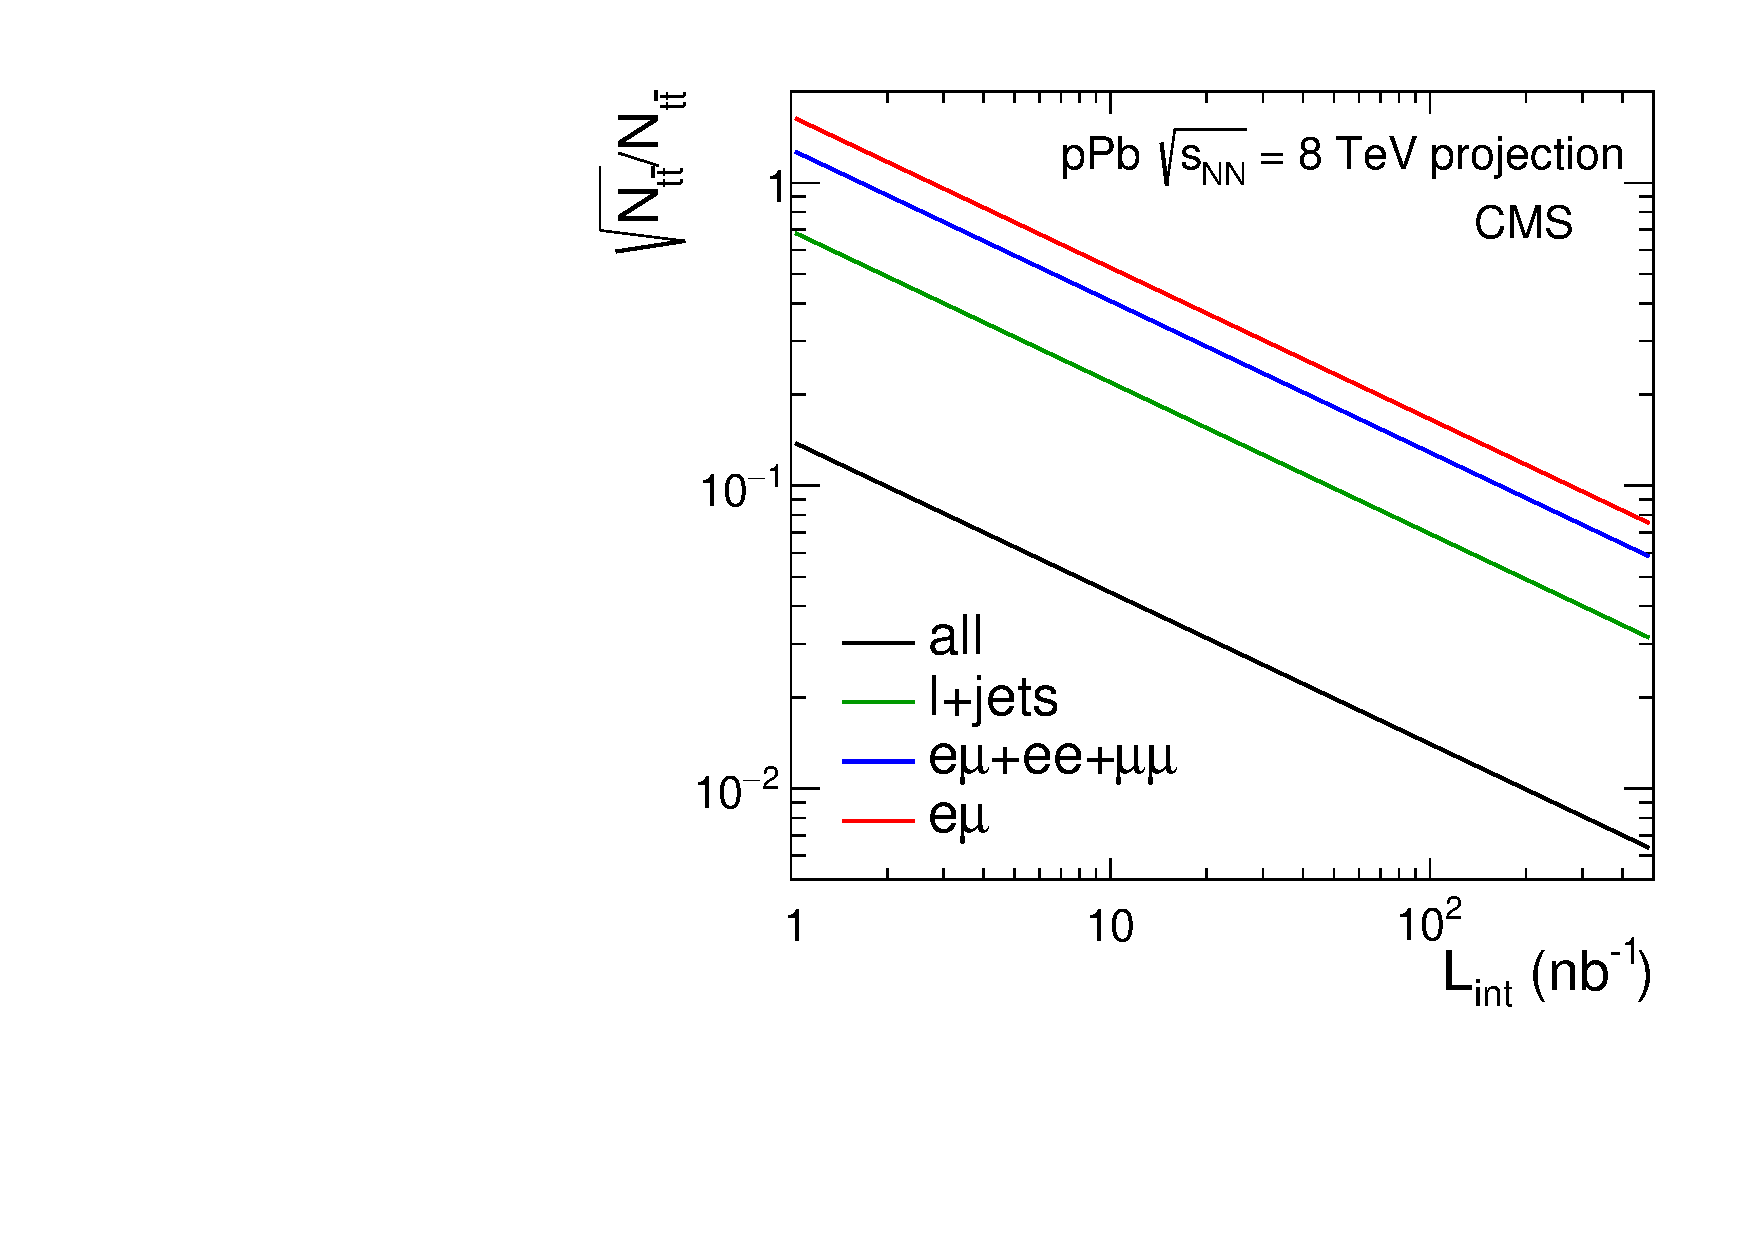
\includegraphics[width= 0.43\textwidth]{figures/top/ProjectedTTbarStatUnc.pdf}
  \caption{Left panel: Expected number of $\mathrm{t}\bar{\mathrm{t}}$ events for several channels in pPb collisions at $\sqrt{s_{\mathrm{NN}}}=8$ TeV as function of total integrated luminosity. Right panel: Corresponding statistical uncertainty as function of total integrated luminosity.
  }
\label{fig:ttPPbProjections}
\end{center}
\end{figure}

The jet energy scale, DY and W+jets physics signal subtraction are the dominating uncertainties for the $\mathrm{t}\bar{\mathrm{t}}$ cross sectio measurements. All these uncertainties can be reduced by measuring them in data. This is only possible if the sampled luminisity is large enough. The evolution of the systematic and statistical uncertainty as function of total integrated luminosity in various pp measurements is shown in Fig. \ref{fig:ttStatSyst}.
\begin{figure}[h!]
\begin{center}
  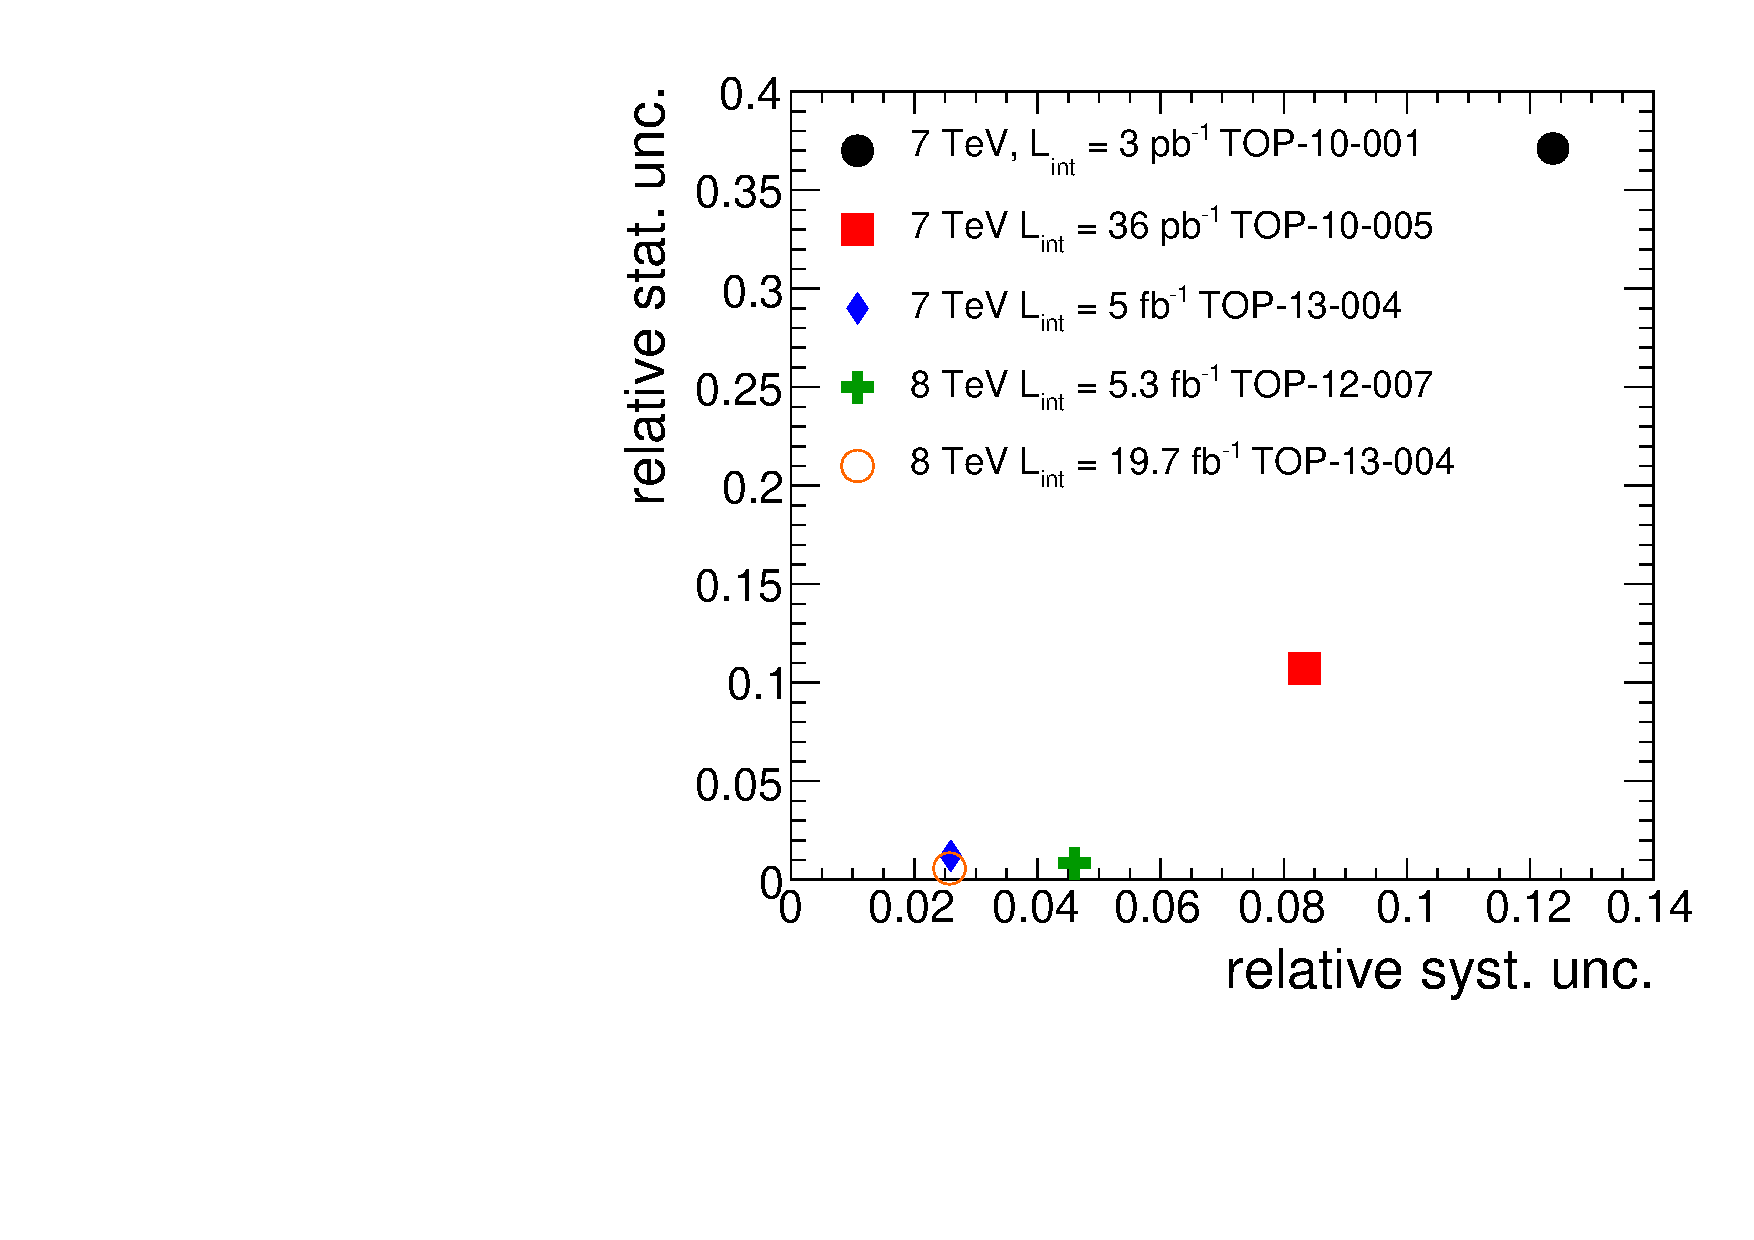
\includegraphics[width= 0.43\textwidth]{figures/top/topToLLXSecUncertaintiesPP.pdf}
  \caption{Evolution of statistical an systematic uncertainty of top pair cross section measurements in the fully leptonic channel in pp collisions at 7 and 8 TeV.
  }
\label{fig:ttStatSyst}
\end{center}
\end{figure}
